\section{Materials and Methods}

\subsection{Data and measurement identity}

We used the CPTAC \texttt{umich} proteomics tables distributed by the
\texttt{cptac} Python package \citep{cptacPkg}. The six retained cohorts have
at least 15 tumor and 15 source-defined nonmalignant samples each:
clear-cell renal-cell carcinoma (CCRCC), lung adenocarcinoma (LUAD), uterine
corpus endometrial carcinoma (UCEC), head-and-neck squamous-cell carcinoma
(HNSCC), lung squamous-cell carcinoma (LSCC), and pancreatic ductal
adenocarcinoma (PDAC). We did not reprocess raw mass-spectrometry files.
The 1{,}191 samples comprise 689 tumors, 496 adjacent-normal samples
and six HNSCC cored-normal samples. The latter have the suffix \texttt{.C};
both these samples and the \texttt{.N} adjacent-normal samples receive label
0, and unsuffixed tumor samples receive label 1. Normal means the source's
nonmalignant tissue category, not a healthy donor. Table~\ref{tab:paircounts}
gives the composition of every cohort.

Patient identities are cohort-scoped sample identifiers after removal of
the applicable \texttt{.N} or HNSCC \texttt{.C} suffix. Unknown suffixes,
duplicate sample IDs, or conflicting identities cause the analysis to
stop. There are 719 patients: 470 with both tissue classes, 219 with tumor
only and 30 with normal only. A patient can contribute more than two
samples; these counts are not a claim of exactly one matched pair per
patient. Earlier versions stripped only \texttt{.N}, misclassified the six
\texttt{.C} samples, and counted 723 patient keys. All three protocols here
use the corrected identities and labels.

The primary matrix contains 8{,}906 stable ENSP accessions present in all
six cohorts, with a consistent gene annotation. We remove accession
version suffixes only after testing stable-accession uniqueness within
each cohort. For the retained intersection, full accession versions also
agree across cohorts. We do not collapse multiple proteins into a gene
name. An earlier gene-indexed intersection retained the first protein per
gene: 1{,}234 of its 9{,}675 gene names selected different stable accessions
across cohorts. As a mapping sensitivity, we retain the 8{,}441 historical
gene names whose first stable accession is consistent in every cohort.
This sensitivity is not independent validation or proof that all isoform
measurement ambiguity has been removed. The intersection of six cohorts was
defined before the outer folds were evaluated. Thus the held-out cohort
contributed its \emph{feature-availability metadata} (which accessions
were measurable), though not its labels, to the fixed feature matrix.
This is a conditional comparison on a shared assay space, not a target-blind
deployment test in which the feature panel is locked before an unknown
cohort arrives.

Abundances are the UMICH reference-intensity-subtracted quantities returned
by the package, not raw total protein signal. We applied no additional
cohort-level normalization or batch correction to the primary matrix.
Missing abundance entries can have multiple mass-spectrometric causes
\citep{LazarMissing}; they are handled by the training-fold imputation below.
The accession map and sample/fold manifest are supplied with the
reproducibility package.

\subsection{Task, features, and model}

The task is tumor versus source-defined nonmalignant tissue. The primary
feature set is the accession-aligned abundance vector. Two comparator
sets use the same samples and accession matrix: a binary missingness mask,
and three per-sample global summaries (mean and median observed abundance,
and detection fraction). These are reference-normalized abundance
summaries, not measurements of raw total intensity. Their performance
differences are predictive comparisons and cannot partition biological
signal into global and protein-specific fractions.

The primary classifier is XGBoost \citep{XGBoost}, with 150 trees,
maximum depth 4, learning rate 0.1, subsample 0.8, column subsample 0.3,
histogram tree method, four threads and log-loss evaluation. No class
weighting, early stopping or nested hyperparameter tuning was used.
The historical hyperparameters were retained; \texttt{random\_state} was
not explicitly set in these XGBoost fits. The corrected analyses used
\texttt{cptac} 1.5.14, XGBoost 3.3.0, NumPy 2.5.0, pandas 3.0.3 and
scikit-learn 1.9.0. Labels, feature identity, grouped folds and parts of
the software environment differ from the historical analysis, so the
revision is not a controlled one-factor ablation of its previous numbers.

\subsection{Evaluation and sensitivity protocols}

Leave-one-cohort-out (LOGO) trains on five cohorts and tests on the sixth,
giving one out-of-cohort prediction per sample. The other protocols are
sample-stratified five-fold cross-validation (\texttt{StratifiedKFold},
\texttt{shuffle=True}, \texttt{random\_state=28}) and true-patient-grouped
five-fold cross-validation (\texttt{GroupKFold}, without shuffling).
The corrected patient-fold manifest replaces, rather than replays, the
invalid historical partition. Joining by cohort and sample ID verifies
the stored fold assignments. Patient-grouped CV and LOGO have zero
true-patient crossings; sample CV assigns samples from 381 patients to
more than one evaluation fold. This is a patient count across the entire
partition, not the mean fraction of pairs split in one train/test fold.

For every primary fit, per-feature medians are estimated on its training
fold, with an entirely missing training feature filled by zero. The same
medians are then applied to the held-out fold. The three global summaries
are computed within each sample before this imputation. All model
comparisons hold the corrected samples and outer LOGO folds fixed.
A deliberately leaky sensitivity uses medians of the entire feature
matrix, including held-out feature values but not held-out labels; it is
a diagnostic, not a recommended protocol. The linear-model sensitivity
uses training-fold median imputation and \texttt{StandardScaler}, followed
by L2 logistic regression (\texttt{lbfgs}, $C=1$, \texttt{max\_iter=500}).
All six linear fits converged. The iteration limit is 500, as in the
executed code, not 1000 as stated by a superseded method-lock writer.

\subsection{Metrics, aggregation and conditional sensitivity}

We report within-cohort area under the receiver operating characteristic
curve (AUROC), ten-bin expected calibration error (ECE), Brier score,
log-loss and accuracy. Equal-cohort macro metrics are the arithmetic mean
of the six within-cohort metrics, including for sample and patient CV.
They are not the mean of the five CV-fold metrics. Pooled metrics are
computed separately after concatenating all 1{,}191 predictions. Pooled
AUROC includes positive--negative pairs from different cohorts whose
scores came from distinct fitted models. It is therefore not the average
of six cohort-transfer AUROCs. Within-cohort sample/patient CV metrics
likewise combine that cohort's out-of-fold predictions.

For an evaluated set of $n$ predictions, $p_i$ is the predicted tumor
probability and $y_i\in\{0,1\}$ is the source-defined tissue label.
Probability bins $S_b$ have width 0.1 on $[0,1]$, closed on the left
and open on the right except for the last bin. ECE is
\begin{equation}\label{eq:ece}
 \mathrm{ECE}=\sum_{b=1}^{10}\frac{|S_b|}{n}
 \left|\overline p_{S_b}-\overline y_{S_b}\right|.
\end{equation}
The bars are the arithmetic means within each nonempty bin. Equation~\ref{eq:ece}
is evaluated separately for each cohort or concatenated prediction set;
empty bins contribute zero. ECE depends on binning and sample composition;
poorer discrimination does not mathematically force overconfidence or an
increase in ECE. We use the Brier score and log-loss as complementary
probability-error summaries (SI Section S2 and Tables~S1--S6).

For a conditional sensitivity analysis, we resample true patients with
replacement within each fixed source cohort, carrying every patient's
stored predictions in all protocols together (2{,}000 draws; seed
20260922). We report the 2.5th--97.5th percentiles of paired protocol
contrasts. These are fixed-prediction mixture-sensitivity ranges, not
confidence intervals for a completely refitted learning algorithm or a
future study. The six cancer/study cohorts are not assumed to be random
exchangeable draws from a population of studies; resampling them alone
would not establish a generic cross-study confidence interval.

Selective prediction ranks the pooled LOGO samples by $|p-0.5|$, retaining
the most confident fraction, with hard label $\mathbf{1}[p\geq0.5]$.
Ties retain source-row order, fixed by the sample manifest. For requested
coverage $c$, the retained count is $\lfloor1191c\rfloor$. We report both
retained accuracy and the cohort composition of that same set. This is
retrospective evaluation of stored predictions, not validation of an
operational abstention threshold.

\subsection{Post-hoc recalibration}

For each outer held-out cohort, we divide the other five cohorts into the
first two and the remaining three in the recorded cohort order. We train
on each group and score the other, then concatenate those inner held-out
predictions. Training-fold imputation is repeated inside each inner fit.
No outer test label enters this procedure. Temperature scaling fits
$T\in[0.05,20]$ by negative-log-likelihood minimization, and Platt scaling
fits logistic regression to the clipped probability logits
(clip $[10^{-7},1-10^{-7}]$, $C=10^6$, maximum 2000 iterations).
These maps are applied to the already-stored outer LOGO probabilities.

The inner predictors train on two or three cohorts while the outer
predictor trains on five. The analysis therefore evaluates this specific
split-half recalibration procedure, not a universal mechanism of
calibration failure under transfer. Each held-out cohort has a different
map; even when each within-cohort map preserves ranking, pooled ranking
can change when those different maps are applied across cohorts.

\subsection{Independent side-study and historical dependencies}

A separate ovarian (OV) side-study uses one cancer type, 12 observed TMT
plexes, and the package's Tumor/Normal annotation: 103 samples (84 tumor,
19 normal) and 10{,}589 protein features, with QC and reference samples
excluded. The abundance--annotation join covers all 103 samples. Its
leave-one-TMT-plex-out protocol (plex-LOGO) uses train-fold medians and the
same XGBoost settings except for explicitly setting
\texttt{random\_state=28}. We retain its recorded result as a separately
scoped historical boundary observation, not as a rerun on the corrected
six-cohort matrix. The source hashes and annotation totals were checked
during integration; full prediction-level replay of OV remains separate.

Historical cohort-identity, permutation, location/scale, residual,
injection, higher-moment and PC-removal diagnostics use the superseded
gene-indexed matrix. Their numerical claims are not retained as evidence
for the corrected primary matrix. The BCM/UMICH three-cohort
dual-platform analysis has a distinct gene mapping and patient join and
also requires its own identity audit before quantitative reuse. The
Supporting Information records the disposition of each dependency, so
these archived experiments are not silently promoted into the new result.

\begin{figure}[tbp]
\centering
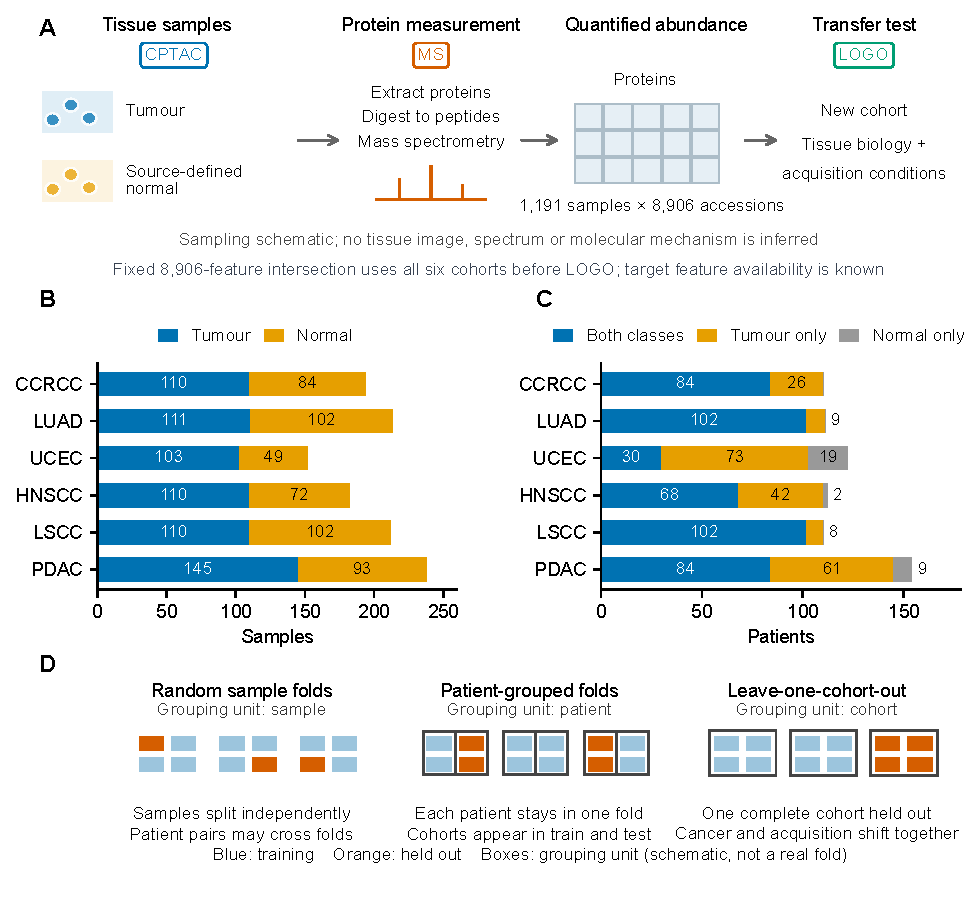
\includegraphics[width=\linewidth]{figures/b28_F0_design.pdf}
\caption{From tissue sampling to cohort transfer. (A) Conceptual path from
tumor and source-defined nonmalignant tissue through mass spectrometry
to the abundance matrix; tissue symbols and peaks are schematic, not
observed histology or spectra. (B) Six cohorts contribute 1,191 samples:
689 tumors and 502 nonmalignant samples, including six HNSCC cored normals.
(C) The 719 true patients include 470 with both tissue classes; some
patients have more than two samples. (D) Sample folds may split a
patient's samples, patient folds keep them together, and LOGO holds out
an entire cancer/study cohort. The blocks illustrate grouping rules,
not actual assignments. The 8,906-feature intersection uses all six
cohorts before LOGO, so target feature availability is known. Cancer
type and study are confounded; the data do not establish one instrument
or one acquisition run per cohort.}
\label{fig:design}
\end{figure}
